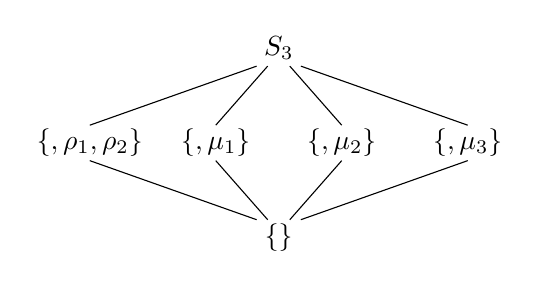
\begin{tikzpicture}[scale=0.8]

\coordinate (top-S3) at (3,1.5);
\coordinate (middle-rho) at (0,0);
\coordinate (middle-mu1) at (2,0);
\coordinate (middle-mu2) at (4,0);
\coordinate (middle-mu3) at (6,0);
\coordinate (bottom-id) at (3,-1.5);

\node at (top-S3) {$S_3$};
\node at (middle-rho) {$\{  \identity, \rho_1, \rho_2\}$};
\node at (middle-mu1) {$\{  \identity, \mu_1\}$};
\node at (middle-mu2) {$\{  \identity, \mu_2 \}$};
\node at (middle-mu3) {$\{  \identity, \mu_3 \}$};
\node at (bottom-id) {$\{ \identity \}$};

\draw  ([yshift=8]middle-rho) -- ([xshift=-10,yshift=-8]top-S3);
\draw  ([yshift=8]middle-mu1) -- ([xshift=-5,yshift=-8]top-S3);
\draw  ([yshift=8]middle-mu2) -- ([xshift=5,yshift=-8]top-S3);
\draw  ([yshift=8]middle-mu3) -- ([xshift=10,yshift=-8]top-S3);

\draw  ([xshift=-10,yshift=8]bottom-id) -- ([yshift=-8]middle-rho);
\draw  ([xshift=-5,yshift=8]bottom-id) -- ([yshift=-8]middle-mu1);
\draw  ([xshift=5,yshift=8]bottom-id) -- ([yshift=-8]middle-mu2);
\draw  ([xshift=10,yshift=8]bottom-id) -- ([yshift=-8]middle-mu3);

\end{tikzpicture}
